\chapter{Analysis and Design}

\section{Synchronous Message Exchange}
The system that we will discuss in this report is called Synchronous Message Exchange

\subsection{Components}
Compared to CSP, a much smaller and simpler set of components are used
to model the process network. In this section, we describe those
components and their

\begin{description}
  \item[Process] A process is an execution unit performing a unit of
    work
  \item[Bus] A bus enables communication between two processes and
    should be considered analogous to buses found in actual
    hardware. As such, they can only be written to or read from once
    per clock cycle.
\end{description}

\subsection{Properties}
The SME model has a number of special properties which influences how
to efficiently represent and execute the network in our implementation.

%\begin{description}
%  \item[Clock cycles] One defining feature of
%    hardware is that all processing is driven by a clock beat. In
%    order to enable fulfillment of this goal we introduce a simulated
%    clock beat in our implementation of SME and thus the defining
%    property of hardware is preserved in the SME model.

%  \item[Global synchronicity] As a consequence of implementing the
%    simulated clock best, all events and communications of the
%    network occurs completely synchronous from the point of view of a
%    process. FIXME

%  \item[Shared nothing] A process is completely
%    autonomous and can only change state through receiving a message
%    on its incoming bus. A process is also self contained in the sense
%\end{description}

\begin{property}[Implicit clock] One defining feature of
    hardware is that all processing is driven by a clock beat. In
    order to enable fulfillment of this goal we introduce a simulated
    clock beat in our implementation of SME and thus the defining
    property of hardware is preserved in the SME model.
\end{property}

\begin{property}[Global synchrony]
  % http://eyes4earth.org/2014/11/synchronicity-or-synchrony/
  \label{synchro}
  As a consequence of implementing the simulated clock best, all
  events and communications of the network occurs completely
  synchronous from the point of view of a process. FIXME
\end{property}

\begin{property}[Shared Nothing]
  \label{noshare}
  A process is completely autonomous and can only change state through
  receiving a message on its incoming bus. A process is also self
  contained in the sense
\end{property}

\subsection{Execution flow}
The execution flow needs to be defined with a focus om preserving the
actual 

The execution cycle of a SME-process 


\begin{figure}
\centering
\includegraphics{figures/execution-cycle}
\label{fig:cycle}
\caption[Execution flow of a SME-process]{The execution cycle of a
  SME process visualized as a hardware clock-cycle. Before every cycle
  data from a input bus is read into the process and after a cycle,
  data is written back to the gate}
\end{figure}

\section{Public API}
The API exposed to the user of the SME library should be designed with
a focus on balancing expressiveness and ability to be easily
understandable....

The API implemented by \cite{vinter2014synchronous} is heavily
dependent of the highly dynamic nature of the Python programming
language used to implement their prototype. Since our implementation
is written in C++ we cannot directly mimic the python API in our
implementation. Given the similarities between SME and CSP it seems
obvious to let us inspire by

\section{Paralellization model}

Using OS-level threads for representing the SME processes was quickly
ruled out during the design process. OS-level threads are severely
limited in that the number of threads a process can have is highly
limited \fxnote{Find reference for number of threads per process} and
switching between OS-level threads is very expensive compared to, for
instance, user-level threads. \cite{sung2002comparative}\fxnote{Find
  more recent citation for the performance of OS vs. user-level threads}.

Using user-level threads, on linux implemented by using the (now
deprecated) \texttt{setjump, longjump} functions or the more current
\texttt{ setcontext, getcontext} functions, is another possible way of
implementing our networks. The notion of a user-level thread is highly
compatible with our concept of a process, namely
\fxnote{finish}. User-level threads is the method that is used to
implement many CSP libraries, including C++CSP2.

One important difference between the CSP and SME execution models is
that CSP is asynchronous and event-driven in nature while SME is, as
previously mentioned, entirely synchronous. This allows us to take a
significantly more simple approach to scheduling threads compared to
C++CSP. A parallel CSP library needs to schedule a process for
execution based on events generated by other processes
\cite{brown2003introduction}. In SME we know that every process needs
to run \fxnote{This needs to be better described} during every ``clock
cycle''. This greatly simplifies our implementation of multi-threaded
SME.

Based on this, we propose an extremely and efficient model for
parallel execution of a SME process network illustrated
in. \fxnote{make figure similar to \Cref{fig:suboptdist}}. The idea is
to start one OS-level thread per available CPU-core and assign a
subset of SME processes to each code. Then, for each iteration of the
SME-network \fxnote{Define ``iteration of SME-network'' as a full
  clock-cycle of the simulated hardware or replace with different
  term}, the controlling thread will start by



\section{Identifying optimal process scheduling}
In order to determine the efficiency of various methods of process
scheduling we need to identify the optimality condition for our
process scheduling. An illustration of our threading model can be seen in
\cref{fig:suboptdist}. The green boxes represents processes while the
red boxes indicates core idle time. Notice, how we by redistributing
the processes across threads could reduce the idle-time of our
cores.

\begin{figure}
\centering
\includegraphics{figures/parallel}
\caption[Proposed SME parallelization model]{Example of suboptimal
  distribution of processes across processing threads. Green blocks
  represents processes while red blocks represents thread idle
  time. Threads are named $p_{i,j}$ where $i$ is the number of the
  thread the process has been assigned to and $f_i$ is the combined
  idle time for each thread. Threads are named $t_i$.}

\label{fig:suboptdist}

\end{figure}

\section{Process orchestration}
As we discussed in the previous section, the primary limiting factor
for our multi-threaded network is an uneven and suboptimal
distribution of processes across CPU-cores. If no attempt is made to
optimize process distribution, the order of process execution will
depend on the order of which processes are defined in the source
code. Due to \cref{noshare} and \cref{synchro} of SME
networks there is no scenario where it would be necessary or
beneficial for a programmer to exercise ultimate control over the
order of process execution. Therefore, maximizing CPU-core utilization
would be an unreasonable burden to put on the programmer, especially
since their optimization efforts would be specific to a certain number
of CPU-cores.

However, the process of orchestrating processes comes at a
computational cost which must weighted against the potential reduction
of core idle-time.

The optimal method and timing of process orchestration depends on the
dynamicity \fxnote{is predictability a better word?} of the work
performed by the network we are executing. A network where each
process performs a fixed amount of work per iteration will only need
to be orchestrated once, while a network where the workload of the
processes are variable will need to be continuously evaluated at
runtime in order to maintain our optimality condition. These various
methods will be discussed for the remainder of this section.

\fxnote{Discuss/investigate problem of
  ``optimization-looping''. Imagine a network where the execution time
  of each process is completely random. This would most likely trigger
  a reorchestration after every iteration which may end up taking more
  CPU-time than the actual process execution.}

\subsection{Round-robin orchestration}
\begin{figure}
\centering
\includegraphics{figures/roundrobin}

\caption[Round-robin orchestration]{Illustration of round-robin
  process orchestration. Progressive iterations are shown as
  increasing color intensity of arrows}

\label{fig:roundrobin}

\end{figure}


Processes will be executed on the first available core as seen in
\cref{fig:roundrobin}


\subsection{One-shot process orchestration}
In this model, we orchestrate the processes in our network as soon as
possible after execution start and

\subsection{Monte Carlo orchestration}
In this approach, we simply randomize the order of the processes. The
main advantage of this approach is that is computationally cheap
compared to

\subsection{Optimization-based orchestration}
Another way to orchestrate the processes is to use a


\subsection{Adaptive process orchestration}
The benefits of using a oneshot orchestration approach diminishes when
we execute process networks where the processes performs a variable
amount of work per iteration. In these kinds of networks, CPU-core
load distribution will gradually become uneven and suboptimal as the
network execution progresses. In order to keep this from happening and
maximize CPU-core utilization, we need to monitor process execution
time and core idle time as the network execution progresses. This is
what we refer to s adaptive orchestration. This approach, however
introduces another trade-off that we need to consider. producing an

\subsection{Adaptive Monte Carlo process orchestration}

\subsection{Adaptive Optimization-based process orchestration}



%%% Local Variables:
%%% mode: latex
%%% TeX-master: "master"
%%% TeX-command-extra-options: "-enable-write18"
%%% End:
